\documentclass[conference]{IEEEtran}
\usepackage[utf8]{inputenc}
\usepackage{amsmath,amssymb,booktabs,graphicx,xcolor,url,multirow}
\usepackage{pgfplots,tikz}
\pgfplotsset{compat=1.17}
\usetikzlibrary{positioning,arrows.meta}
\newcommand{\pend}[1]{\textcolor{red}{#1}}

\begin{document}
\title{Recall First: A Tiny, DSP-Assisted Detector of Safety Sounds\\for Deaf and Hard-of-Hearing People}
\author{\IEEEauthorblockN{Anonymous}\IEEEauthorblockA{Anonymous institution}}
\maketitle

\begin{abstract}
Sound-awareness devices for deaf and hard-of-hearing (DHH) people must not miss a fire alarm,
yet they are usually evaluated with clip-level accuracy on curated clips, which hides both
missed events and false alarms. We build and evaluate, under one locked protocol on real public
recordings, a detector of six safety sounds (smoke/fire alarm, siren, doorbell, knock, baby cry,
car horn) small enough for a \$5 microcontroller. A CNN14 teacher fine-tuned on AudioSet strong
labels is distilled into depthwise-separable CNNs of 7--239\,KB (int8). The 239\,KB student keeps
90\% of the teacher's event recall at 0.1 false alarm per hour (32.4\% vs.\ 35.8\%) and beats the
3.7\,M-parameter YAMNet on every clip-level metric. A DSP simulation ablation shows that mixing
real home backgrounds helps (+4.4 points) while synthetic room, occlusion and microphone models do
not help on close-mic test audio. Finally, we fuse the students with classical detectors derived
from the physics of each sound (Goertzel-style tone detection, ISO~8201 beep cycling, pitch-sweep
tracking, onset regularity, harmonicity) under a recall-first protocol (95\% target for alarms and
sirens): \pend{[phase 5 result]}.
\end{abstract}

\section{Introduction}
For a DHH person living alone, a missed smoke alarm is a safety failure, while a false alert is
an annoyance. Commercial and research sound-awareness systems~\cite{homesound,soundwatch} use
neural audio classifiers and report clip-level accuracy. Two gaps follow. First, accuracy on
rare sounds is uninformative: on our test set, a detector that never fires is 98.5\% accurate.
Second, false alarms, the reason users silence such devices, are rarely measured per hour of
real audio. We therefore evaluate event recall at a fixed false-alarm rate per hour, with
thresholds fixed on separate tuning data, on 910 real event clips and 37\,h of real negative
audio, and later switch to a recall-first operating point.

Contributions: (i) a locked public benchmark and protocol for DHH safety-sound detection with
false alarms per hour of real home audio; (ii) a distilled int8 student family (7--239\,KB) for
the ESP32-S3 and its size/recall trade-off; (iii) an ablation of DSP-based training simulation;
(iv) physics-based DSP detectors fused with the network under a recall-first protocol.

\section{Data and protocol}
\textbf{Sources.} Real events come from the AudioSet strong-label evaluation set~\cite{audioset,strong}
(all six classes) and FSD50K evaluation~\cite{fsd50k} (siren, doorbell, knock, car horn). Real
negatives are AudioSet evaluation clips with none of the six classes (21.8\,h, varied) and SINS
home recordings~\cite{sins} (15.6\,h, one home; sessions held out from training). Clips whose
labels may hide a target (``Alarm'', ``Emergency vehicle'', ``Crying, sobbing'') are excluded
from negatives. Training uses the AudioSet strong-label training set (80\% of videos), AudioSet
balanced train and FSD50K development; tuning uses the remaining 20\% of videos, FSD50K
validation and separate SINS sessions. The test set (Table~\ref{tab:data}) was hashed and locked
before any model was trained.

\begin{table}[t]\centering\caption{Locked test set}\label{tab:data}
\begin{tabular}{lrrrrrr}\toprule
 & alarm & siren & doorb. & knock & baby & horn \\ \midrule
event clips & 63 & 283 & 98 & 136 & 64 & 282 \\ \bottomrule
\end{tabular}\\[2pt]
\footnotesize negatives: 7{,}928 AudioSet clips (21.8\,h) + 5{,}622 SINS segments (15.6\,h)
\end{table}

\textbf{Event-level metric.} Every detector scores each class every 0.5\,s from the last 2\,s of
audio (causal). An alert fires when a score crosses the class threshold, then the class is silent
for 10\,s. Labelled events of one class closer than 5\,s form one occurrence, detected if an
alert falls between its onset and $\max(\text{offset}, \text{onset}+2\,\text{s})$. False alarms
are alerts on negative audio, per hour. Thresholds are set on the tuning negatives for 0.1 and
1 false alarm per hour (FA/h) and applied unchanged to test. We report macro recall over classes.

\section{System}
\begin{figure}[t]\centering
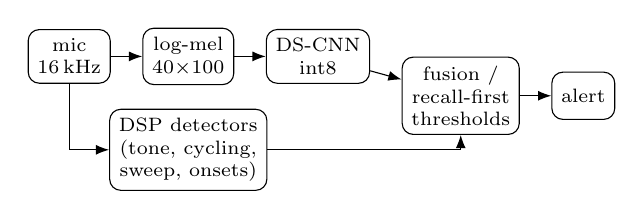
\begin{tikzpicture}[font=\scriptsize, node distance=3mm and 4mm, b/.style={draw, rounded corners, align=center, minimum height=6mm}]
\node[b] (mic) {mic\\16\,kHz};
\node[b, right=of mic] (fe) {log-mel\\40$\times$100};
\node[b, right=of fe] (cnn) {DS-CNN\\int8};
\node[b, below=of fe] (dsp) {DSP detectors\\(tone, cycling,\\sweep, onsets)};
\node[b, right=of cnn, yshift=-5mm] (fu) {fusion /\\recall-first\\thresholds};
\node[b, right=of fu] (out) {alert};
\draw[-Latex] (mic) -- (fe); \draw[-Latex] (fe) -- (cnn); \draw[-Latex] (mic) |- (dsp);
\draw[-Latex] (cnn) -- (fu); \draw[-Latex] (dsp) -| (fu); \draw[-Latex] (fu) -- (out);
\end{tikzpicture}
\caption{On-device pipeline. The teacher (CNN14) is used only in training.}\label{fig:sys}
\end{figure}

\textbf{Teacher.} CNN14 (16\,kHz, AudioSet-pretrained, 80\,M parameters)~\cite{panns} with a new
6-way head initialised from the mean of each class's AudioSet head rows, fine-tuned end to end
on 2\,s windows with SpecAugment~\cite{specaug} (AdamW, one-cycle, lr $10^{-4}$, 15k steps).

\textbf{Students.} DS-CNN~\cite{dscnn} on 40 log-mel bands $\times$ 100 frames (512-point FFT,
20\,ms hop, 50--8000\,Hz): a $3{\times}3$ stride-2 convolution, $N$ depthwise-separable blocks
(the second strided), frequency mean, time max+mean, linear. Sizes S/M/L/XL have widths
32/64/128/192 and 4/4/5/6 blocks. Students are trained on simulated examples generated on the fly
with $0.5\,\mathrm{BCE}(\text{labels}) + 0.5\,\mathrm{BCE}(\text{teacher})$~\cite{kd}, the
teacher scoring the same simulated example. Int8: batch norm folded, weights symmetric per
channel, activations asymmetric per tensor (TFLite scheme~\cite{tflm}).

\textbf{DSP training simulation} (cumulative configurations): (B) mixing a real SINS background
at SNR $\mathcal{U}(-5,25)$\,dB and a random level; (C) a statistical room impulse
response~\cite{polack}: direct path, image-source early reflections with amplitude $d/(d+\Delta)$,
and a Gaussian tail decaying as $e^{-6.9t/T_{60}}$ in four bands, scaled to the
direct-to-reverberant ratio $(r_c/d)^2$ with critical distance $r_c=0.057\sqrt{V/T_{60}}$~\cite{kuttruff};
(D) transmission through a door or wall (first/second-order low-pass, 300--1500\,Hz, mass law);
(E) an INMP441-like microphone (port high-pass, $\pm4$\,dB high shelf, self-noise, clipping).

\section{Results}
\textbf{Baselines and teacher} (Table~\ref{tab:main}). Zero-shot YAMNet~\cite{yamnet} and CNN14
reach only 14--17\% event recall at 0.1\,FA/h. Fine-tuning CNN14 doubles it (35.8\%), while its
clip-level AP barely moves (0.717$\to$0.731): clip-level metrics hide the strict-false-alarm
regime that matters for a safety device.

\begin{table}[t]\centering\caption{Test results. Event recall at 0.1 / 1 FA/h (thresholds from
tuning) and clip-level AUC / AP. Students distilled; int8 unless noted.}\label{tab:main}
\setlength{\tabcolsep}{3.5pt}
\begin{tabular}{lrrrrr}\toprule
Model & Size & @0.1 & @1 & AUC & AP \\ \midrule
YAMNet zero-shot & 3.7\,M p. & 13.9 & 55.5 & .948 & .635 \\
CNN14 zero-shot & 80\,M p. & 16.6 & 66.1 & .974 & .717 \\
CNN14 fine-tuned (teacher) & 80\,M p. & \textbf{35.8} & \textbf{66.8} & \textbf{.978} & \textbf{.731} \\ \midrule
Student S & 6.7\,KB & 11.1 & 42.7 & .950 & .490 \\
Student M & 21.5\,KB & 22.7 & 53.0 & .962 & .592 \\
Student L & 93\,KB & 27.8 & 57.1 & .965 & .650 \\
Student XL & 239\,KB & 28.6 & 59.5 & .965 & .661 \\
Student XL (float) & & 32.4 & 59.3 & .965 & .667 \\ \bottomrule
\end{tabular}\end{table}

\textbf{Simulation ablation} (Table~\ref{tab:sim}, student M, hard labels, two runs each).
Mixing real home backgrounds is the only consistent gain (+4.4 points at 1\,FA/h on test, +3.5
on tuning). Room, occlusion and microphone simulation add nothing measurable, and room simulation
alone lowers strict-budget recall; fine-tuning the teacher on configuration D instead of raw
clips also lowers its tuning recall (62.5\% vs.\ 65.8\%), so the distillation teacher, chosen on
tuning, is the raw-data one. Our test events are mostly close-mic YouTube and Freesound
recordings; a far-field test set is needed to judge far-field simulation (a limitation).

\begin{table}[t]\centering\caption{Simulation ablation: macro event recall (\%), mean of two runs}\label{tab:sim}
\begin{tabular}{lrrr}\toprule
Training data & test @0.1 & test @1 & tune @1 \\ \midrule
A raw clips & 22.3 & 45.5 & 43.3 \\
B + home background mixing & 22.1 & 49.9 & 46.8 \\
C + room reverberation & 16.9 & 49.5 & 47.3 \\
D + door/wall occlusion & 22.1 & 49.3 & 47.3 \\
E + microphone model & 23.7 & 49.1 & 47.1 \\ \bottomrule
\end{tabular}\end{table}

\textbf{Distillation and size.} Distillation lifts student M from 22.1\% to 28.1\% at 0.1\,FA/h
and from 49.3\% to 52.5\% at 1\,FA/h (float; tuning agrees). Recall grows with size
(Fig.~\ref{fig:size}); XL keeps 90\% of the teacher's strict-budget recall with 1/330 of its
parameters, and beats YAMNet at both budgets and on every clip-level metric. Int8 is lossless at
1\,FA/h for L and XL and costs 0--6 points at 0.1\,FA/h. A PCEN front end~\cite{pcen} is worse
than log-mel here (18.2\% vs.\ 28.1\% at 0.1\,FA/h for M). Real home audio (SINS) produces at
most 0.15 FA/h for every model; the budget is spent on the varied AudioSet negatives.

\begin{figure}[t]\centering
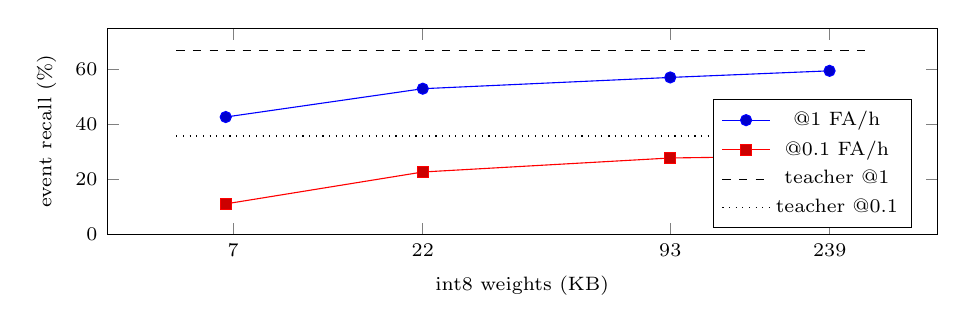
\begin{tikzpicture}\begin{axis}[width=\columnwidth, height=4.2cm, xmode=log, xlabel={int8 weights (KB)},
ylabel={event recall (\%)}, legend pos=south east, legend style={font=\scriptsize}, ymin=0, ymax=75,
xtick={7,21.5,93,239}, xticklabels={7,22,93,239}, tick label style={font=\scriptsize}, label style={font=\scriptsize}]
\addplot+[mark=*] coordinates {(6.7,42.7)(21.5,53.0)(93,57.1)(238.7,59.5)}; \addlegendentry{@1 FA/h}
\addplot+[mark=square*] coordinates {(6.7,11.1)(21.5,22.7)(93,27.8)(238.7,28.6)}; \addlegendentry{@0.1 FA/h}
\addplot[dashed, domain=5:300] {66.8}; \addlegendentry{teacher @1}
\addplot[dotted, domain=5:300] {35.8}; \addlegendentry{teacher @0.1}
\end{axis}\end{tikzpicture}
\caption{Recall of int8 students vs.\ size.}\label{fig:size}\end{figure}

\textbf{Recall-first operation with DSP detectors.} \pend{[Phase 5: recall-first protocol (95\%
target alarm/siren, 90\% others, set on tuning); per-class choice among network, smoothed
network, network OR calibrated DSP, logistic fusion; test recall reached and FA/h cost; loud-sound
safety net.]} The DSP detectors are derived from the physics of each sound: a narrowband tone
in 2--5\,kHz that dominates the low band at a fixed frequency and switches on and off (ISO~8201
signal~\cite{iso8201}; per-bin peak prominence, i.e.\ a Goertzel-style~\cite{goertzel} tone test
on all bins); a sustained tonal peak in 500--1800\,Hz with a smooth sweep of more than 150\,Hz
(siren); a tonal onset that keeps ringing and decays (chime); broadband onsets with regular
80--700\,ms spacing (knock); voicing with $f_0$ in 300--650\,Hz, harmonics 1--3 and no
sub-harmonic energy, with pitch movement (baby cry); a loud steady tone that does not decay (horn);
and a class-agnostic level jump over a tracked noise floor (safety net). All run causally with a
minimum-follower noise floor and cost under 5\,ms per second of audio on a desktop CPU.

\textbf{Deployment.} \pend{[export: real int8 TFLite sizes, ops, agreement with the simulated
int8 model.]} Measuring latency and power on the ESP32-S3 is future work.

\section{Conclusion}
Under a strict, locked, event-level protocol on real recordings, a 239\,KB distilled int8 CNN
retains most of a large teacher's ability to catch safety sounds and outperforms widely used
on-device models; physics-based DSP detectors \pend{[phase 5 conclusion]}. Limitations: one home
for real negatives, close-mic test events, two runs per ablation configuration, and no on-device
measurements yet.

\bibliographystyle{IEEEtran}
\bibliography{refs}
\end{document}
